
%% Work Day Generalized
\workday{Day-of-the-Week, Month Day}{mm/dd}
%% Argument 1: for the section title and the TOC.
%% Argument 2: used for tagging deliverables/receivables with a date in their respective lists.

  %% Quick list of plans for the day, whether you get to them or not.
  \todotoday  %% A simple command to prevent writing the same initial sentence everyday
  \stit  %% Redefine \begin{itemize} command
    \itm Create a template.
    \itm Send to prospective users.
    \itm  %% Redefine of itemize/enumerate environment \item command
  \enit  %% Redefine \end{itemize} command

  %% First project of the day (experiment = project)
  \experiment{prjA}  %% Please see packages/labbook.pdf for full explanation of use.
    General notes about a project can go here that would not apply to a specific subproject of the project.

    \subexperiment{Atask1}  %% (subexperiment = subproject) Please see packages/labbook.pdf for full explanation of use.
    \stit
      \itm Notes on subproject.
      \itm 
    \enit

    %% Defines a referencable process, which may or maynot be related to the project.
    \process{Project A Process 1}{prjA1}
    %% Arg 1: Process Title, for use in TOC and Process List
    %% Arg 2: Label, for use when referenceing the process in your notes. Example: \ref{procs:prjA1}
    \sten  %% Redefine \begin{enumerate}
      \itm Step 1.
      \itm Step 2.
      \itm Success Criteria: Always!
    \enen

    \subexperiment{Atask2}
      Notes do not have to be itemized.
  
      %% Defines a deliverable wrt project/subproject.
      \deliv{A Task 2}{Atask2}
      %% Arg 1: Title, for use in TOC and Delivery List
      %% Arg 2: Label, for use when referenceing the process in your notes. Example: \ref{deliv:Atask2}
      Delivery notes:
      \stit
        \itm Who
        \itm What
        \itm Why
        \itm ...
      \enit

%% Next work day
\workday{Monday, January 1}{01/01}
  \todotoday
  \stit
    \itm Sleep.
  \enit
  \experiment{prjA}

    \receive{Project A Baseline 1}{Abase1}
    %% Arg 1: Title, for use in TOC and Receivable List
    %% Arg 2: Label, for use when referenceing the process in your notes. Example: \ref{receive:Abase1}
      From Som E. One. It fixes problem X.

    %% Can combine projects and subprojects, but still have it indexed seperately.
    \subexperiment[Task 1 Performance,Atask1,APerf]{Performance of Task 1}  %% Please see packages/labbook.pdf for further details.
    \stit
      \itm Analyze performance of task in \nameref{receive:Abase1}. % \nameref can be used for process/deliv/receive/fix because they are "sections"
      \itm Increased! Yay!
    \enit
    \process{How to Build PDF from \LaTeX}{buildPDFLatex}
    \sten
      \itm Complete current note-taking session. 
      \itm Spell-check your recently edited notes, if you care. At Odyssey you will have to ask for hunspell to be installed. 
           Example: $>$ hunspell -t mmdd.tex
      \itm Execute pdflatex on main tex file. Example: $>$ pdflatex year.tex
      \itm Resolve any errors or warnings.
      \itm Execute makeindex on main idx file to generate index. Example: $>$ makeindex year.idx
      \itm Resolve any errors or warnings.
      \itm If you have a bibliography, execute bibtex on the main aux file. Example: $>$ bibtex year.aux
      \itm Resolve any errors or warnings.
      \itm Execute pdflatex twice. The second time ensures all references are included. Example: $>$ pdflatex year.tex
      \itm Open and enjoy a PDF version of your notes.
    \enen
  \experiment{prjB}
    \subexperiment{Btask1}
    \stit
      \itm Added following algorithm \cite{bk:gps_misra}: % Here is an example of a bibliograph citation. Basic LaTeX rules apply.
      %% Here is an example equation. Basic LaTeX rules apply.
      \begin{equation}\label{eq:EqOfB}
        1B = 2B - 1B
      \end{equation}
      \itm Memory usage increased.
    \enit
    \subexperiment{Btask2}
    \stit
      \itm See results in Figure \ref{fig:B2}
      \itm Eqn. \ref{eq:EqOfB} doesn't work very well for this task.
      %% Here is an example figure. Basic LaTeX rules apply.
      \begin{figure}[H]
        \begin{center}
        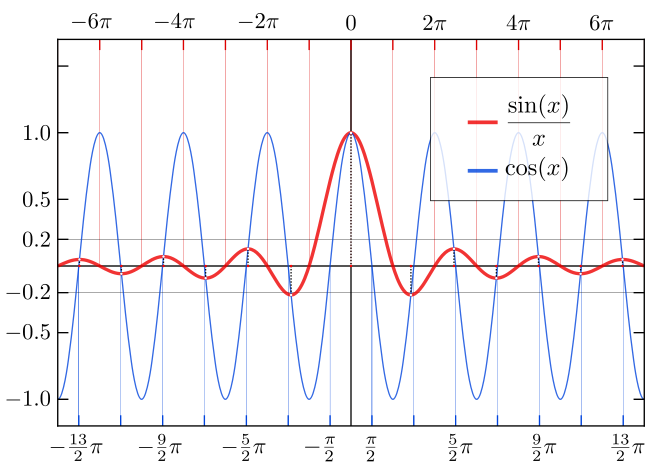
\includegraphics[width=1.0\textwidth]{year/fig/picture}
        \caption{Performance of B2}
        \label{fig:B2}
        \end{center}
      \end{figure}
      \itm Finally figured out why it wont compile! See Fix \ref{fix:simulinkIosrcHeader}.
    \enit
    %% Real example of how I use the fix-list
    \fix{Error: expected =, ;, ], ) or \_\_attribute\_\_ before `Simulink\_Class'}{simulinkIosrcHeader}
    %% Arg 1: Title, for use in TOC and Fix List
    %% Arg 2: Label, for use when referenceing the fix in your notes. Example: \ref{fix:simulinkIosrcHeader}
      Error occurs during build in a Simulink auto-generated header file included in a trick generated
      io\_src file. Note the io\_src files will be a *.c instead of an expected *.cpp. That is the problem, it needs
      be a *.cpp. For example:
%% Example verbatim section, very useful for code snippets. Becareful of page run-off if you care.
\begin{verbatim}
  In file included from io_src/io_comp_az_el_OrionSim.c:53:
  /home/garnerd1/simulink/comp_az_el_OrionSim.h:47: error: expected  =, ;, ], ), __attribute__ before "Simulink_OrionSimClass"
  make: *** [/home/garnerd1/simulink/object_Linux_4.1_25_x86_64/io_comp_az_el_OrionSim.c]
\end{verbatim}
      To make the io\_src file a *.cpp you need to add the following Trick header to the comments of the *.h
      in question:
\begin{verbatim}
/*
 * PURPOSE: (The sRFComModel Class (sModel) the main class of the sRFCom Model.)
 * LANGUAGE: (CPP)
 * PROGRAMMERS: ((Unknown) (LMSSC) (2011))
 */
\end{verbatim}

\workday{Tuesday, January 2}{01/02}
  \todotoday
  \stit
    \itm Demonstrate reference-able process.
  \enit
  \experiment{prjA}
    \subexperiment{Atask1}
      Performed \nameref{procs:prjA1} again...
      \deliv{A Task 1}{Atask1}
  \experiment{prjB}
    \subexperiment{Btask1}
    \stit
      \itm Table \ref{tab:B1} shows the results.
      %% Here is an example table. Basic LaTeX rules apply.
      \begin{table}[H]
      \begin{center}
      {\bf \caption{Statistical Comparison} \label{tab:B1}}
      \vspace{5pt}
      \begin{tabular}{|c|r|r|r|r|} \hline
        Region        & Bias          & Data Std     & Truth Std     & Count (--) \\ \hline
        2             &  0.0003739548 & 0.001657984  & 0.001295738   &  2401      \\
        13            & -0.0005374600 & 0.001601039  & 0.001827648   & 17601      \\
        10            & -0.0016334410 & 0.001609881  & 0.001630779   &  8801      \\
        5             &  0.0001470492 & 0.001590097  & 0.001318719   &  6801      \\
        3             &  0.0009888838 & 0.001594697  & 0.001327540   &  6401      \\
        0             &  0.0014194210 & 0.001606638  & 0.001251639   &  1801      \\ \hline
      \end{tabular}
      \end{center}
      \end{table}
      \itm Good comparison!
    \enit
    
